\documentclass[border=3pt,tikz]{standalone}
\usepackage{amsmath}
\usepackage{wasysym}
\tikzset{%
  ddash/.style={
    dash pattern={on 6pt off 4pt},
  }
}
\usetikzlibrary{calc}
\usetikzlibrary{arrows.meta} % for arrow size	
\usetikzlibrary{shapes.geometric}

\begin{document}
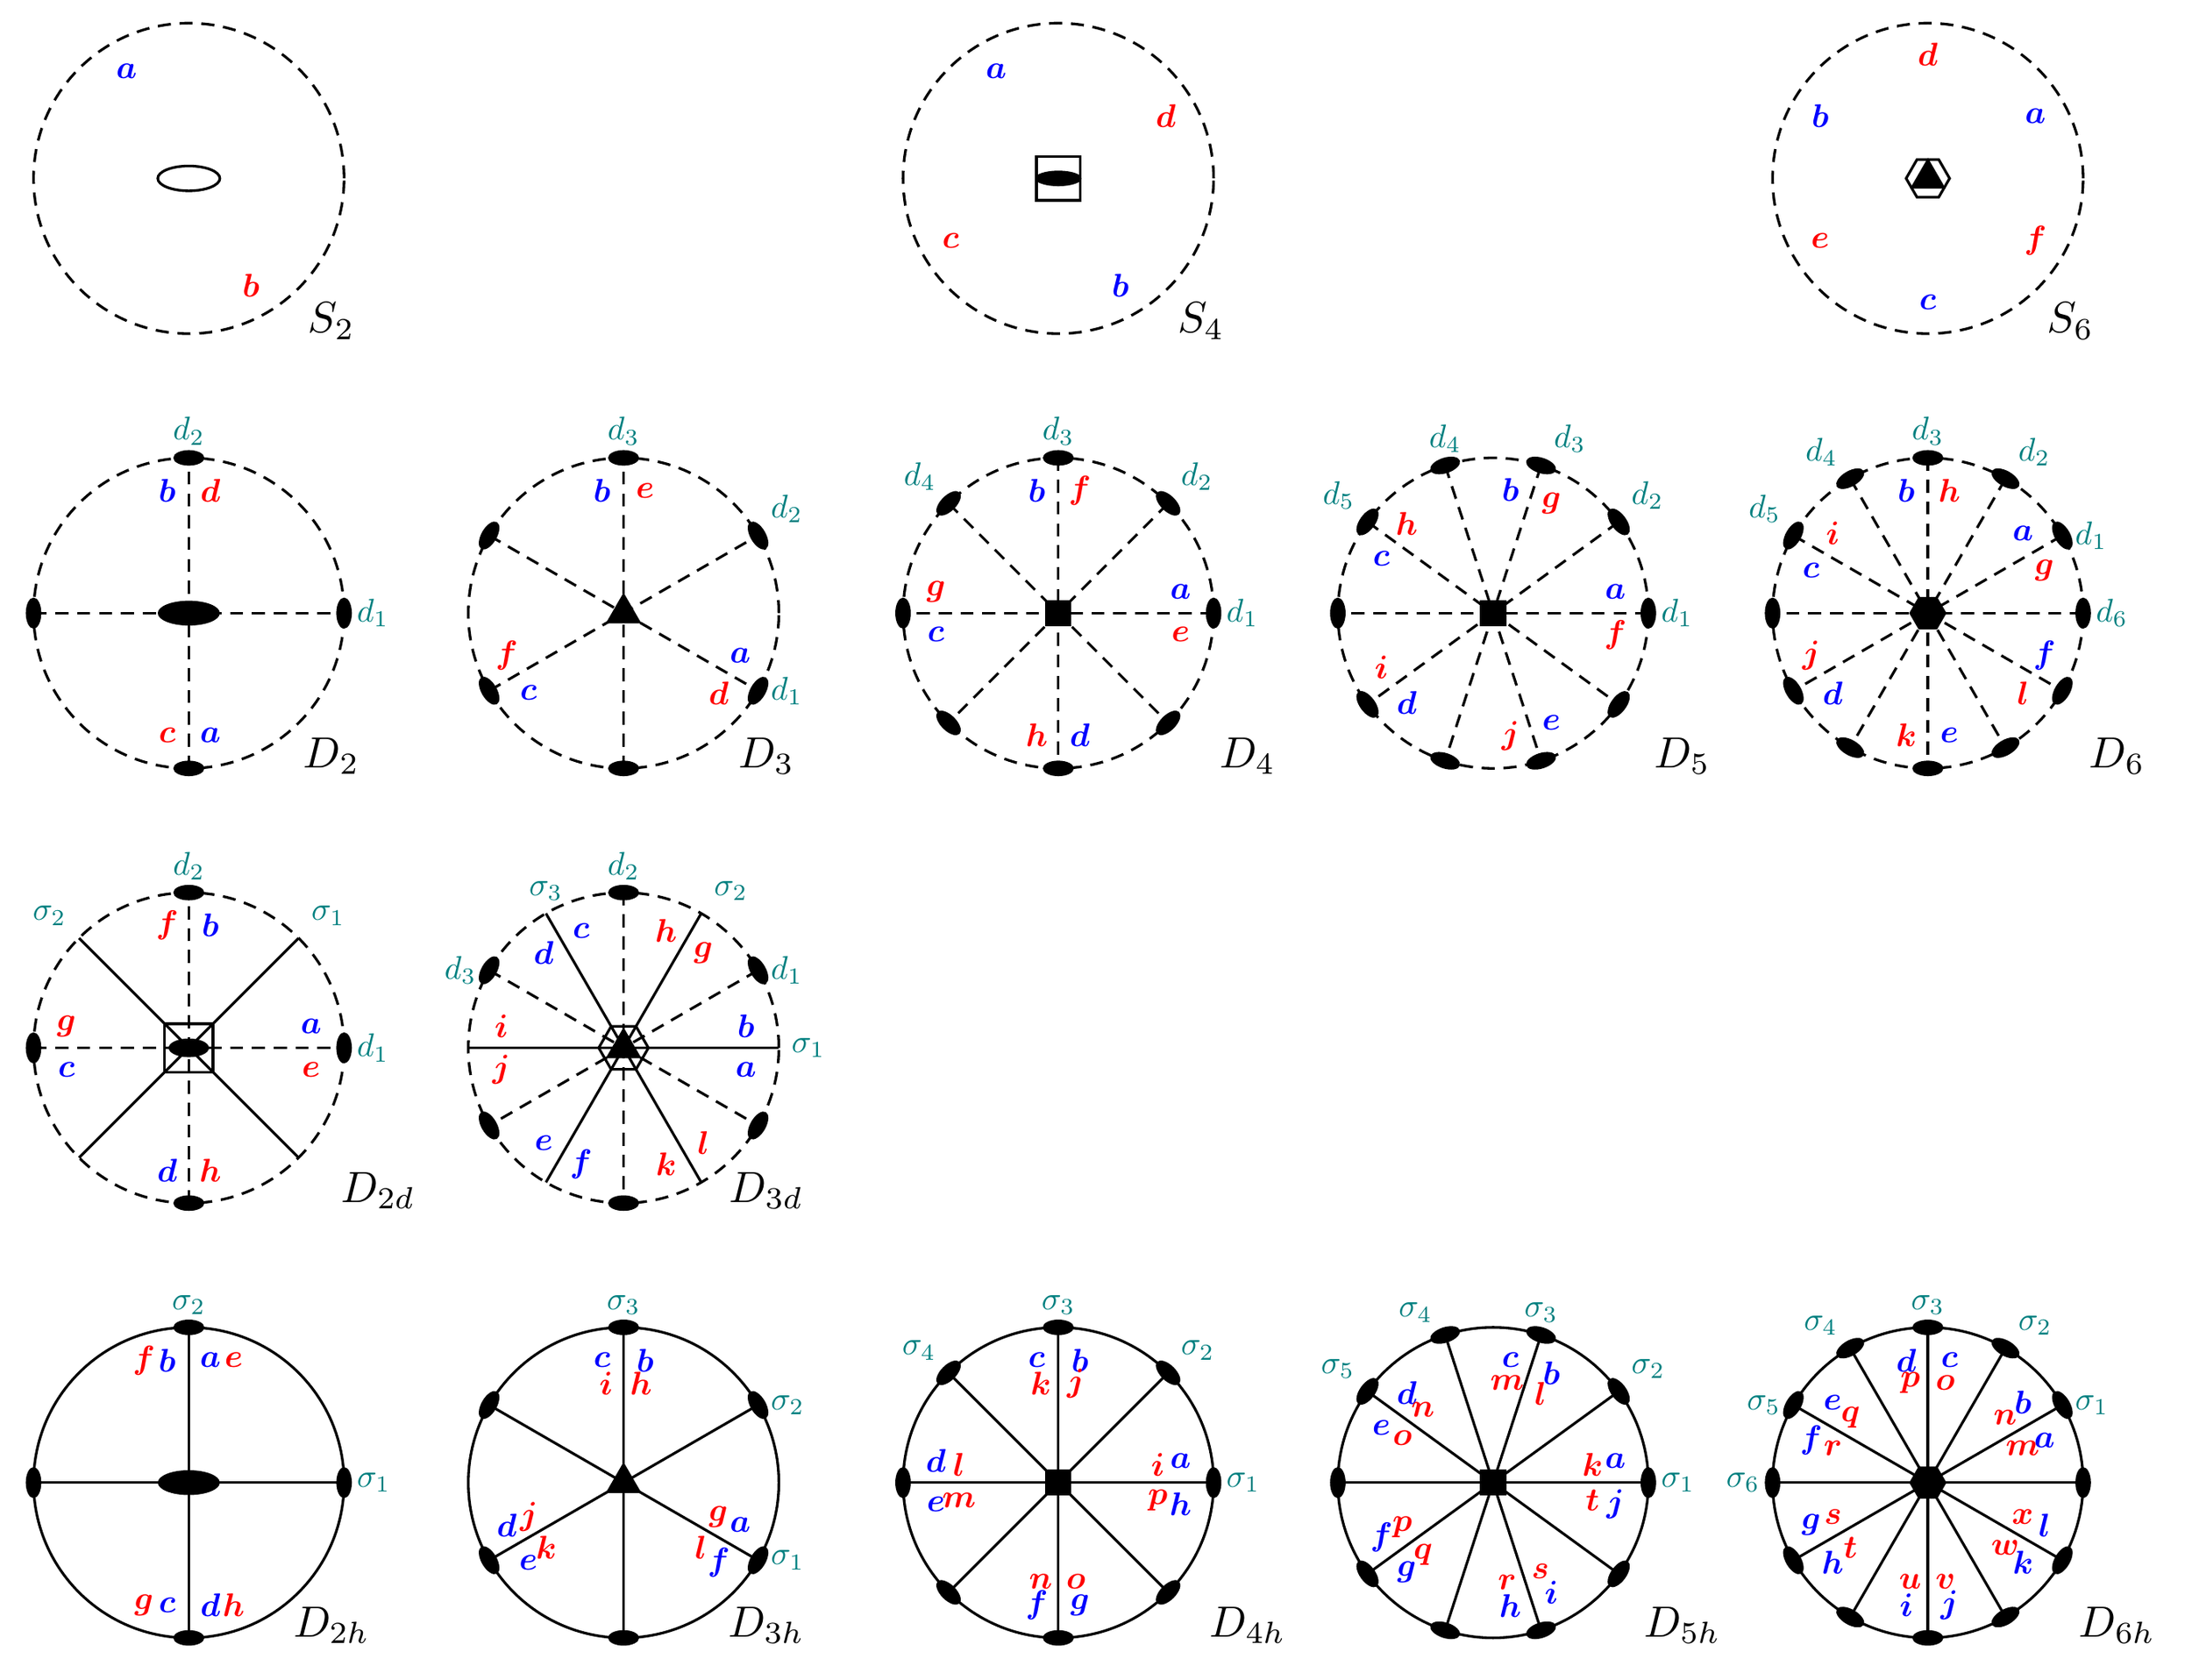
\begin{tikzpicture}[scale=2.5, extended line/.style={shorten >=-#1,shorten <=-#1},
    extended line/.default=1cm]

 

    \begin{scope}[xshift=2.8cm]
        \def\Ra{1.3};
        \def\Rb{0.8};
        \draw[ddash, very thick](0,0) circle (1);
        \node[scale=2] at ({\Ra*cos(315)}, {\Ra*sin(315)}) {$S_2$};
        \draw[very thick] (0,0) ellipse (0.2 and 0.08);
        \node[blue, scale=1.5] at ({\Rb*cos(120)}, {\Rb*sin(120)}) {$\boldsymbol{a}$};
        \node[red, scale=1.5] at ({\Rb*cos(300)}, {\Rb*sin(300)}) {$\boldsymbol{b}$};
    \end{scope}

    \begin{scope}[xshift=8.4cm]
        \def\Ra{1.3};
        \def\Rb{0.8};
        \draw[ddash, very thick](0,0) circle (1);
        \node[scale=2] at ({\Ra*cos(315)}, {\Ra*sin(315)}) {$S_4$};
        \node[draw, very thick, minimum size=1cm,regular polygon,regular polygon sides=4] at (0, 0) {};
        \fill[] (0,0) ellipse (0.15 and 0.05);
        \node[blue, scale=1.5] at ({\Rb*cos(120)}, {\Rb*sin(120)}) {$\boldsymbol{a}$};
        \node[red, scale=1.5] at ({\Rb*cos(210)}, {\Rb*sin(210)}) {$\boldsymbol{c}$};
        \node[blue, scale=1.5] at ({\Rb*cos(300)}, {\Rb*sin(300)}) {$\boldsymbol{b}$};
        \node[red, scale=1.5] at ({\Rb*cos(30)}, {\Rb*sin(30)}) {$\boldsymbol{d}$};
    \end{scope}

    \begin{scope}[xshift=14.0cm]
        \def\Ra{1.3};
        \def\Rb{0.8};
        \draw[ddash, very thick](0,0) circle (1);
        \node[scale=2] at ({\Ra*cos(315)}, {\Ra*sin(315)}) {$S_6$};
        \node[draw, very thick, minimum size=0.7cm,regular polygon,regular polygon sides=6] at (0, 0) {};
        \node[fill,minimum size=0.4cm,regular polygon,regular polygon sides=3] at (0, 0) {};
        \node[blue, scale=1.5] at ({\Rb*cos(30)}, {\Rb*sin(30)}) {$\boldsymbol{a}$};
        \node[red, scale=1.5] at ({\Rb*cos(90)}, {\Rb*sin(90)}) {$\boldsymbol{d}$};
        \node[blue, scale=1.5] at ({\Rb*cos(150)}, {\Rb*sin(150)}) {$\boldsymbol{b}$};
        \node[red, scale=1.5] at ({\Rb*cos(210)}, {\Rb*sin(210)}) {$\boldsymbol{e}$};
        \node[blue, scale=1.5] at ({\Rb*cos(270)}, {\Rb*sin(270)}) {$\boldsymbol{c}$};
        \node[red, scale=1.5] at ({\Rb*cos(330)}, {\Rb*sin(330)}) {$\boldsymbol{f}$};
    \end{scope}

    \begin{scope}[xshift=2.8cm, yshift=-2.8cm]
        \def\Ra{1.3};
        \def\Rb{0.8};
        \draw[ddash, very thick](0,0) circle (1);
        \node[scale=2] at ({\Ra*cos(315)}, {\Ra*sin(315)}) {$D_{2}$};
        \fill[] (0,0) ellipse (0.2 and 0.08);
        \fill[] (1,0) ellipse (0.05 and 0.1);
        \fill[] (0,1) ellipse (0.1 and 0.05);
        \fill[] (-1,0) ellipse (0.05 and 0.1);
        \fill[] (0,-1) ellipse (0.1 and 0.05);
        \draw[very thick, ddash] (-1, 0) -- (1, 0) node [teal, scale=1.5, right] {$d_1$};
        \draw[very thick, ddash] (0, -1) -- (0, 1) node [teal, scale=1.5, above] {$d_2$};
        \node[red, scale=1.5] at ({\Rb*cos(80)}, {\Rb*sin(80)}) {$\boldsymbol{d}$};
        \node[blue, scale=1.5] at ({\Rb*cos(100)}, {\Rb*sin(100)}) {$\boldsymbol{b}$};
        \node[red, scale=1.5] at ({\Rb*cos(260)}, {\Rb*sin(260)}) {$\boldsymbol{c}$};
        \node[blue, scale=1.5] at ({\Rb*cos(280)}, {\Rb*sin(280)}) {$\boldsymbol{a}$};
    \end{scope}

    \begin{scope}[xshift=5.6cm, yshift=-2.8cm]
        \def\Ra{1.3};
        \def\Rb{0.8};
        \draw[ddash, very thick](0,0) circle (1);
        \node[scale=2] at ({\Ra*cos(315)}, {\Ra*sin(315)}) {$D_{3}$};
        \node[fill,minimum size=0.5cm,regular polygon,regular polygon sides=3] at (0, 0) {};
        \fill[shift={({cos(30)}, {sin(30)})}, rotate=30] (0,0) ellipse (0.05 and 0.1);
        \fill[shift={({cos(90)}, {sin(90)})}, rotate=90] (0,0) ellipse (0.05 and 0.1);
        \fill[shift={({cos(150)}, {sin(150)})}, rotate=150] (0,0) ellipse (0.05 and 0.1);
        \fill[shift={({cos(210)}, {sin(210)})}, rotate=210] (0,0) ellipse (0.05 and 0.1);
        \fill[shift={({cos(270)}, {sin(270)})}, rotate=270] (0,0) ellipse (0.05 and 0.1);
        \fill[shift={({cos(330)}, {sin(330)})}, rotate=330] (0,0) ellipse (0.05 and 0.1);
        \draw[very thick, ddash] (0, -1) -- (0, 1) node [teal, scale=1.5, above] {$d_3$};
        \draw[very thick, ddash] ({cos(210)}, {sin(210)})  -- ({cos(30)}, {sin(30)}) node [teal, scale=1.5, above right] {$d_2$};
        \draw[very thick, ddash] ({cos(150)}, {sin(150)}) -- ({cos(330)}, {sin(330)}) node [teal, scale=1.5, right] {$d_1$};
        \node[red, scale=1.5] at ({\Rb*cos(80)}, {\Rb*sin(80)}) {$\boldsymbol{e}$};
        \node[blue, scale=1.5] at ({\Rb*cos(100)}, {\Rb*sin(100)}) {$\boldsymbol{b}$};
        \node[red, scale=1.5] at ({\Rb*cos(200)}, {\Rb*sin(200)}) {$\boldsymbol{f}$};
        \node[blue, scale=1.5] at ({\Rb*cos(220)}, {\Rb*sin(220)}) {$\boldsymbol{c}$};
        \node[red, scale=1.5] at ({\Rb*cos(320)}, {\Rb*sin(320)}) {$\boldsymbol{d}$};
        \node[blue, scale=1.5] at ({\Rb*cos(340)}, {\Rb*sin(340)}) {$\boldsymbol{a}$};
    \end{scope}


    \begin{scope}[xshift=8.4cm, yshift=-2.8cm]
        \def\Ra{1.3};
        \def\Rb{0.8};
        \draw[ddash, very thick](0,0) circle (1);
        \node[scale=2] at ({\Ra*cos(315) + 0.3}, {\Ra*sin(315)}) {$D_{4}$};
        \node[fill,minimum size=0.6cm,regular polygon,regular polygon sides=4] at (0, 0) {};
        \fill[shift={({cos(0)}, {sin(0)})}, rotate=0] (0,0) ellipse (0.05 and 0.1);
        \fill[shift={({cos(45)}, {sin(45)})}, rotate=45] (0,0) ellipse (0.05 and 0.1);
        \fill[shift={({cos(90)}, {sin(90)})}, rotate=90] (0,0) ellipse (0.05 and 0.1);
        \fill[shift={({cos(135)}, {sin(135)})}, rotate=135] (0,0) ellipse (0.05 and 0.1);
        \fill[shift={({cos(180)}, {sin(180)})}, rotate=180] (0,0) ellipse (0.05 and 0.1);
        \fill[shift={({cos(225)}, {sin(225)})}, rotate=225] (0,0) ellipse (0.05 and 0.1);
        \fill[shift={({cos(270)}, {sin(270)})}, rotate=270] (0,0) ellipse (0.05 and 0.1);
        \fill[shift={({cos(315)}, {sin(315)})}, rotate=315] (0,0) ellipse (0.05 and 0.1);
        \draw[very thick, ddash] ({cos(0)}, {sin(0)}) node [right, teal, scale=1.5]{$d_1$} -- ({cos(180)}, {sin(180)});
        \draw[very thick, ddash] ({cos(45)}, {sin(45)}) node [above right, teal, scale=1.5]{$d_2$}-- ({cos(225)}, {sin(225)});
        \draw[very thick, ddash] ({cos(90)}, {sin(90)}) node [above, teal, scale=1.5]{$d_3$}-- ({cos(270)}, {sin(270)});
        \draw[very thick, ddash] ({cos(135)}, {sin(135)}) node [above left, teal, scale=1.5]{$d_4$}-- ({cos(315)}, {sin(315)});
        \node[blue, scale=1.5] at ({\Rb*cos(10)}, {\Rb*sin(10)}) {$\boldsymbol{a}$};
        \node[red, scale=1.5] at ({\Rb*cos(350)}, {\Rb*sin(350)}) {$\boldsymbol{e}$};
        \node[red, scale=1.5] at ({\Rb*cos(80)}, {\Rb*sin(80)}) {$\boldsymbol{f}$};
        \node[blue, scale=1.5] at ({\Rb*cos(100)}, {\Rb*sin(100)}) {$\boldsymbol{b}$};
        \node[red, scale=1.5] at ({\Rb*cos(170)}, {\Rb*sin(170)}) {$\boldsymbol{g}$};
        \node[blue, scale=1.5] at ({\Rb*cos(190)}, {\Rb*sin(190)}) {$\boldsymbol{c}$};
        \node[red, scale=1.5] at ({\Rb*cos(260)}, {\Rb*sin(260)}) {$\boldsymbol{h}$};
        \node[blue, scale=1.5] at ({\Rb*cos(280)}, {\Rb*sin(280)}) {$\boldsymbol{d}$};
    \end{scope}

       \begin{scope}[xshift=11.2cm, yshift=-2.8cm]
        \def\Ra{1.3};
        \def\Rb{0.8};
        \draw[ddash, very thick](0,0) circle (1);
        \node[scale=2] at ({\Ra*cos(315) + 0.3}, {\Ra*sin(315)}) {$D_{5}$};
        \node[fill,minimum size=0.6cm,regular polygon,regular polygon sides=4] at (0, 0) {};
        \fill[shift={({cos(0)}, {sin(0)})}, rotate=0] (0,0) ellipse (0.05 and 0.1);
        \fill[shift={({cos(36)}, {sin(36)})}, rotate=36] (0,0) ellipse (0.05 and 0.1);
        \fill[shift={({cos(72)}, {sin(72)})}, rotate=72] (0,0) ellipse (0.05 and 0.1);
        \fill[shift={({cos(108)}, {sin(108)})}, rotate=108] (0,0) ellipse (0.05 and 0.1);
        \fill[shift={({cos(144)}, {sin(144)})}, rotate=144] (0,0) ellipse (0.05 and 0.1);
        \fill[shift={({cos(180)}, {sin(180)})}, rotate=180] (0,0) ellipse (0.05 and 0.1);
        \fill[shift={({cos(216)}, {sin(216)})}, rotate=216] (0,0) ellipse (0.05 and 0.1);
        \fill[shift={({cos(252)}, {sin(252)})}, rotate=252] (0,0) ellipse (0.05 and 0.1);
        \fill[shift={({cos(288)}, {sin(288)})}, rotate=288] (0,0) ellipse (0.05 and 0.1);
        \fill[shift={({cos(324)}, {sin(324)})}, rotate=324] (0,0) ellipse (0.05 and 0.1);

        \draw[very thick, ddash] ({cos(0)}, {sin(0)}) node [right, teal, scale=1.5]{$d_1$} -- ({cos(180)}, {sin(180)});
        \draw[very thick, ddash] ({cos(36)}, {sin(36)}) node [above right, teal, scale=1.5]{$d_2$}-- ({cos(216)}, {sin(216)});
        \draw[very thick, ddash] ({cos(72)}, {sin(72)}) node [above right, teal, scale=1.5]{$d_3$}-- ({cos(252)}, {sin(252)});
        \draw[very thick, ddash] ({cos(108)}, {sin(108)}) node [above, teal, scale=1.5]{$d_4$}-- ({cos(288)}, {sin(288)});
        \draw[very thick, ddash] ({cos(144)}, {sin(144)}) node [above left, teal, scale=1.5]{$d_5$}-- ({cos(324)}, {sin(324)});
        \node[blue, scale=1.5] at ({\Rb*cos(10)}, {\Rb*sin(10)}) {$\boldsymbol{a}$};
        \node[blue, scale=1.5] at ({\Rb*cos(82)}, {\Rb*sin(82)}) {$\boldsymbol{b}$};
        \node[blue, scale=1.5] at ({\Rb*cos(154)}, {\Rb*sin(154)}) {$\boldsymbol{c}$};
        \node[blue, scale=1.5] at ({\Rb*cos(226)}, {\Rb*sin(226)}) {$\boldsymbol{d}$};
        \node[blue, scale=1.5] at ({\Rb*cos(298)}, {\Rb*sin(298)}) {$\boldsymbol{e}$};        

        \node[red, scale=1.5] at ({\Rb*cos(350)}, {\Rb*sin(350)}) {$\boldsymbol{f}$};
        \node[red, scale=1.5] at ({\Rb*cos(62)}, {\Rb*sin(62)}) {$\boldsymbol{g}$};
        \node[red, scale=1.5] at ({\Rb*cos(134)}, {\Rb*sin(134)}) {$\boldsymbol{h}$};
        \node[red, scale=1.5] at ({\Rb*cos(206)}, {\Rb*sin(206)}) {$\boldsymbol{i}$};
        \node[red, scale=1.5] at ({\Rb*cos(278)}, {\Rb*sin(278)}) {$\boldsymbol{j}$};

    \end{scope}

    \begin{scope}[xshift=14.0cm, yshift=-2.8cm]
        \def\Ra{1.3};
        \def\Rb{0.8};
        \draw[ddash, very thick](0,0) circle (1);
        \node[scale=2] at ({\Ra*cos(315) + 0.3}, {\Ra*sin(315)}) {$D_{6}$};
        \node[fill,minimum size=0.6cm,regular polygon,regular polygon sides=6] at (0, 0) {};
        \fill[shift={({cos(0)}, {sin(0)})}, rotate=0] (0,0) ellipse (0.05 and 0.1);
        \fill[shift={({cos(30)}, {sin(30)})}, rotate=30] (0,0) ellipse (0.05 and 0.1);
        \fill[shift={({cos(60)}, {sin(60)})}, rotate=60] (0,0) ellipse (0.05 and 0.1);
        \fill[shift={({cos(90)}, {sin(90)})}, rotate=90] (0,0) ellipse (0.05 and 0.1);
        \fill[shift={({cos(120)}, {sin(120)})}, rotate=120] (0,0) ellipse (0.05 and 0.1);
        \fill[shift={({cos(150)}, {sin(150)})}, rotate=150] (0,0) ellipse (0.05 and 0.1);
        \fill[shift={({cos(180)}, {sin(180)})}, rotate=180] (0,0) ellipse (0.05 and 0.1);
        \fill[shift={({cos(210)}, {sin(210)})}, rotate=210] (0,0) ellipse (0.05 and 0.1);
        \fill[shift={({cos(240)}, {sin(240)})}, rotate=240] (0,0) ellipse (0.05 and 0.1);
        \fill[shift={({cos(270)}, {sin(270)})}, rotate=270] (0,0) ellipse (0.05 and 0.1);
        \fill[shift={({cos(300)}, {sin(300)})}, rotate=300] (0,0) ellipse (0.05 and 0.1);
        \fill[shift={({cos(330)}, {sin(330)})}, rotate=330] (0,0) ellipse (0.05 and 0.1);
        \draw[very thick, ddash] ({cos(0)}, {sin(0)}) node [teal, right, scale=1.5] {$d_6$}-- ({cos(180)}, {sin(180)});
        \draw[very thick, ddash] ({cos(30)}, {sin(30)}) node [teal, right, scale=1.5] {$d_1$} -- ({cos(210)}, {sin(210)});
        \draw[very thick, ddash] ({cos(60)}, {sin(60)}) node [teal, above right, scale=1.5] {$d_2$}-- ({cos(240)}, {sin(240)});
        \draw[very thick, ddash] ({cos(90)}, {sin(90)}) node [teal, above, scale=1.5] {$d_3$} -- ({cos(270)}, {sin(270)});
        \draw[very thick, ddash] ({cos(120)}, {sin(120)}) node [teal, above left, scale=1.5] {$d_4$}-- ({cos(300)}, {sin(300)});
        \draw[very thick, ddash] ({cos(150)}, {sin(150)}) node [teal, above left, scale=1.5] {$d_5$}-- ({cos(330)}, {sin(330)});
        \node[red, scale=1.5] at ({\Rb*cos(20)}, {\Rb*sin(20)}) {$\boldsymbol{g}$};
        \node[blue, scale=1.5] at ({\Rb*cos(40)}, {\Rb*sin(40)}) {$\boldsymbol{a}$};
        \node[red, scale=1.5] at ({\Rb*cos(80)}, {\Rb*sin(80)}) {$\boldsymbol{h}$};
        \node[blue, scale=1.5] at ({\Rb*cos(100)}, {\Rb*sin(100)}) {$\boldsymbol{b}$};
        \node[red, scale=1.5] at ({\Rb*cos(140)}, {\Rb*sin(140)}) {$\boldsymbol{i}$};
        \node[blue, scale=1.5] at ({\Rb*cos(160)}, {\Rb*sin(160)}) {$\boldsymbol{c}$};
        \node[red, scale=1.5] at ({\Rb*cos(200)}, {\Rb*sin(200)}) {$\boldsymbol{j}$};
        \node[blue, scale=1.5] at ({\Rb*cos(220)}, {\Rb*sin(220)}) {$\boldsymbol{d}$};
        \node[red, scale=1.5] at ({\Rb*cos(260)}, {\Rb*sin(260)}) {$\boldsymbol{k}$};
        \node[blue, scale=1.5] at ({\Rb*cos(280)}, {\Rb*sin(280)}) {$\boldsymbol{e}$};
        \node[red, scale=1.5] at ({\Rb*cos(320)}, {\Rb*sin(320)}) {$\boldsymbol{l}$};
        \node[blue, scale=1.5] at ({\Rb*cos(340)}, {\Rb*sin(340)}) {$\boldsymbol{f}$};
    \end{scope}


    \begin{scope}[xshift=2.8cm, yshift=-5.6cm]
        \def\Ra{1.3};
        \def\Rb{0.8};
        \draw[ddash, very thick](0,0) circle (1);
        \node[scale=2] at ({\Ra*cos(315) + 0.3}, {\Ra*sin(315)}) {$D_{2d}$};
        \fill[] (0,0) ellipse (0.13 and 0.06);
        \node[draw, very thick, minimum size=1.1cm,regular polygon,regular polygon sides=4] at (0, 0) {};
        \fill[] (1,0) ellipse (0.05 and 0.1);
        \fill[] (0,1) ellipse (0.1 and 0.05);
        \fill[] (-1,0) ellipse (0.05 and 0.1);
        \fill[] (0,-1) ellipse (0.1 and 0.05);
        \draw[very thick, ddash] (-1, 0) -- (1, 0) node [teal, right, scale=1.5] {$d_1$};
        \draw[very thick, ddash] (0, -1) -- (0, 1) node [teal, above, scale=1.5] {$d_2$};
        \draw[very thick] ({cos(45)}, {sin(45)}) node [teal, above right, scale=1.5] {$\sigma_1$}-- ({cos(225)}, {sin(225)});
        \draw[very thick] ({cos(135)}, {sin(135)}) node [teal, above left, scale=1.5] {$\sigma_2$}-- ({cos(315)}, {sin(315)});
        \node[red, scale=1.5] at ({\Rb*cos(350)}, {\Rb*sin(350)}) {$\boldsymbol{e}$};
        \node[blue, scale=1.5] at ({\Rb*cos(10)}, {\Rb*sin(10)}) {$\boldsymbol{a}$};
        \node[blue, scale=1.5] at ({\Rb*cos(80)}, {\Rb*sin(80)}) {$\boldsymbol{b}$};
        \node[red, scale=1.5] at ({\Rb*cos(100)}, {\Rb*sin(100)}) {$\boldsymbol{f}$};
        \node[red, scale=1.5] at ({\Rb*cos(170)}, {\Rb*sin(170)}) {$\boldsymbol{g}$};
        \node[blue, scale=1.5] at ({\Rb*cos(190)}, {\Rb*sin(190)}) {$\boldsymbol{c}$};
        \node[blue, scale=1.5] at ({\Rb*cos(260)}, {\Rb*sin(260)}) {$\boldsymbol{d}$};
        \node[red, scale=1.5] at ({\Rb*cos(280)}, {\Rb*sin(280)}) {$\boldsymbol{h}$};
    \end{scope}

    \begin{scope}[xshift=5.6cm, yshift=-5.6cm]
        \def\Ra{1.3};
        \def\Rb{0.8};
        \draw[ddash, very thick](0,0) circle (1);
        \node[scale=2] at ({\Ra*cos(315)}, {\Ra*sin(315)}) {$D_{3d}$};
        \node[fill,minimum size=0.6cm,regular polygon,regular polygon sides=3] at (0, 0) {};
        \node[draw, very thick, minimum size=0.8cm,regular polygon,regular polygon sides=6] at (0, 0) {};
        \fill[shift={({cos(30)}, {sin(30)})}, rotate=30] (0,0) ellipse (0.05 and 0.1);
        \fill[shift={({cos(90)}, {sin(90)})}, rotate=90] (0,0) ellipse (0.05 and 0.1);
        \fill[shift={({cos(150)}, {sin(150)})}, rotate=150] (0,0) ellipse (0.05 and 0.1);
        \fill[shift={({cos(210)}, {sin(210)})}, rotate=210] (0,0) ellipse (0.05 and 0.1);
        \fill[shift={({cos(270)}, {sin(270)})}, rotate=270] (0,0) ellipse (0.05 and 0.1);
        \fill[shift={({cos(330)}, {sin(330)})}, rotate=330] (0,0) ellipse (0.05 and 0.1);
        \draw[very thick] ({cos(0)}, {sin(0)}) node [teal, right, scale=1.5] {$\sigma_1$}-- ({cos(180)}, {sin(180)});
        \draw[very thick, ddash] ({cos(30)}, {sin(30)}) node [teal, right, scale=1.5] {$d_1$}-- ({cos(210)}, {sin(210)});
        \draw[very thick] ({cos(60)}, {sin(60)}) node [teal, above right, scale=1.5] {$\sigma_2$}-- ({cos(240)}, {sin(240)});
        \draw[very thick, ddash] ({cos(90)}, {sin(90)}) node [teal, above, scale=1.5] {$d_2$} -- ({cos(270)}, {sin(270)});
        \draw[very thick] ({cos(120)}, {sin(120)}) node [teal, above, scale=1.5] {$\sigma_3$}-- ({cos(300)}, {sin(300)});
        \draw[very thick, ddash] ({cos(150)}, {sin(150)}) node [teal, left, scale=1.5] {$d_3$}-- ({cos(330)}, {sin(330)});
        \node[blue, scale=1.5] at ({\Rb*cos(350)}, {\Rb*sin(350)}) {$\boldsymbol{a}$};
        \node[blue, scale=1.5] at ({\Rb*cos(10)}, {\Rb*sin(10)}) {$\boldsymbol{b}$};
        \node[red, scale=1.5] at ({\Rb*cos(50)}, {\Rb*sin(50)}) {$\boldsymbol{g}$};
        \node[red, scale=1.5] at ({\Rb*cos(70)}, {\Rb*sin(70)}) {$\boldsymbol{h}$};
        \node[blue, scale=1.5] at ({\Rb*cos(110)}, {\Rb*sin(110)}) {$\boldsymbol{c}$};
        \node[blue, scale=1.5] at ({\Rb*cos(130)}, {\Rb*sin(130)}) {$\boldsymbol{d}$};
        \node[red, scale=1.5] at ({\Rb*cos(170)}, {\Rb*sin(170)}) {$\boldsymbol{i}$};
        \node[red, scale=1.5] at ({\Rb*cos(190)}, {\Rb*sin(190)}) {$\boldsymbol{j}$};
        \node[blue, scale=1.5] at ({\Rb*cos(230)}, {\Rb*sin(230)}) {$\boldsymbol{e}$};
        \node[blue, scale=1.5] at ({\Rb*cos(250)}, {\Rb*sin(250)}) {$\boldsymbol{f}$};
        \node[red, scale=1.5] at ({\Rb*cos(290)}, {\Rb*sin(290)}) {$\boldsymbol{k}$};
        \node[red, scale=1.5] at ({\Rb*cos(310)}, {\Rb*sin(310)}) {$\boldsymbol{l}$};
    \end{scope}


    \begin{scope}[xshift=2.8cm, yshift=-8.4cm]
        \def\Ra{1.3};
        \def\Rb{0.8};
        \draw[very thick](0,0) circle (1);
        \node[scale=2] at ({\Ra*cos(315)}, {\Ra*sin(315)}) {$D_{2h}$};
        \fill[] (0,0) ellipse (0.2 and 0.08);
        \fill[] (1,0) ellipse (0.05 and 0.1);
        \fill[] (0,1) ellipse (0.1 and 0.05);
        \fill[] (-1,0) ellipse (0.05 and 0.1);
        \fill[] (0,-1) ellipse (0.1 and 0.05);
        \draw[very thick] (-1, 0) -- (1, 0) node [teal, right, scale=1.5] {$\sigma_1$};
        \draw[very thick] (0, -1) -- (0, 1) node [teal, above, scale=1.5] {$\sigma_2$};
        \node[blue, scale=1.5] at ({\Rb*cos(80)}, {\Rb*sin(80)}) {$\boldsymbol{a}$};
        \node[blue, scale=1.5] at ({\Rb*cos(100)}, {\Rb*sin(100)}) {$\boldsymbol{b}$};
        \node[blue, scale=1.5] at ({\Rb*cos(260)}, {\Rb*sin(260)}) {$\boldsymbol{c}$};
        \node[blue, scale=1.5] at ({\Rb*cos(280)}, {\Rb*sin(280)}) {$\boldsymbol{d}$};
        \node[red, scale=1.5] at ({\Rb*cos(80)+0.15}, {\Rb*sin(80)}) {$\boldsymbol{e}$};
        \node[red, scale=1.5] at ({\Rb*cos(100)-0.15}, {\Rb*sin(100)}) {$\boldsymbol{f}$};
        \node[red, scale=1.5] at ({\Rb*cos(260)-0.15}, {\Rb*sin(260)}) {$\boldsymbol{g}$};
        \node[red, scale=1.5] at ({\Rb*cos(280)+0.15}, {\Rb*sin(280)}) {$\boldsymbol{h}$};
    \end{scope}

    \begin{scope}[xshift=5.6cm, yshift=-8.4cm]
        \def\Ra{1.3};
        \def\Rb{0.8};
        \def\Rc{0.65};
        \draw[very thick](0,0) circle (1);
        \node[scale=2] at ({\Ra*cos(315)}, {\Ra*sin(315)}) {$D_{3h}$};
        \node[fill,minimum size=0.5cm,regular polygon,regular polygon sides=3] at (0, 0) {};
        \fill[shift={({cos(30)}, {sin(30)})}, rotate=30] (0,0) ellipse (0.05 and 0.1);
        \fill[shift={({cos(90)}, {sin(90)})}, rotate=90] (0,0) ellipse (0.05 and 0.1);
        \fill[shift={({cos(150)}, {sin(150)})}, rotate=150] (0,0) ellipse (0.05 and 0.1);
        \fill[shift={({cos(210)}, {sin(210)})}, rotate=210] (0,0) ellipse (0.05 and 0.1);
        \fill[shift={({cos(270)}, {sin(270)})}, rotate=270] (0,0) ellipse (0.05 and 0.1);
        \fill[shift={({cos(330)}, {sin(330)})}, rotate=330] (0,0) ellipse (0.05 and 0.1);
        \draw[very thick] (0, -1) -- (0, 1) node [teal, above, scale=1.5] {$\sigma_3$};
        \draw[very thick] ({cos(30)}, {sin(30)}) node [teal, right, scale=1.5] {$\sigma_2$}-- ({cos(210)}, {sin(210)});
        \draw[very thick] ({cos(150)}, {sin(150)}) -- ({cos(330)}, {sin(330)}) node [teal, right, scale=1.5] {$\sigma_1$};;
        \node[blue, scale=1.5] at ({\Rb*cos(80)}, {\Rb*sin(80)}) {$\boldsymbol{b}$};
        \node[blue, scale=1.5] at ({\Rb*cos(100)}, {\Rb*sin(100)}) {$\boldsymbol{c}$};
        \node[blue, scale=1.5] at ({\Rb*cos(200)}, {\Rb*sin(200)}) {$\boldsymbol{d}$};
        \node[blue, scale=1.5] at ({\Rb*cos(220)}, {\Rb*sin(220)}) {$\boldsymbol{e}$};
        \node[blue, scale=1.5] at ({\Rb*cos(320)}, {\Rb*sin(320)}) {$\boldsymbol{f}$};
        \node[blue, scale=1.5] at ({\Rb*cos(340)}, {\Rb*sin(340)}) {$\boldsymbol{a}$};
        \node[red, scale=1.5] at ({\Rc*cos(340)}, {\Rc*sin(340)}) {$\boldsymbol{g}$};
        \node[red, scale=1.5] at ({\Rc*cos(80)}, {\Rc*sin(80)}) {$\boldsymbol{h}$};
        \node[red, scale=1.5] at ({\Rc*cos(100)}, {\Rc*sin(100)}) {$\boldsymbol{i}$};
        \node[red, scale=1.5] at ({\Rc*cos(200)}, {\Rc*sin(200)}) {$\boldsymbol{j}$};
        \node[red, scale=1.5] at ({\Rc*cos(220)}, {\Rc*sin(220)}) {$\boldsymbol{k}$};
        \node[red, scale=1.5] at ({\Rc*cos(320)}, {\Rc*sin(320)}) {$\boldsymbol{l}$};
    \end{scope}


    \begin{scope}[xshift=8.4cm, yshift=-8.4cm]
        \def\Ra{1.3};
        \def\Rb{0.8};
        \def\Rc{0.65};
        \draw[very thick](0,0) circle (1);
        \node[scale=2] at ({\Ra*cos(315)+0.3}, {\Ra*sin(315)}) {$D_{4h}$};
        \node[fill,minimum size=0.6cm,regular polygon,regular polygon sides=4] at (0, 0) {};
        \fill[shift={({cos(0)}, {sin(0)})}, rotate=0] (0,0) ellipse (0.05 and 0.1);
        \fill[shift={({cos(45)}, {sin(45)})}, rotate=45] (0,0) ellipse (0.05 and 0.1);
        \fill[shift={({cos(90)}, {sin(90)})}, rotate=90] (0,0) ellipse (0.05 and 0.1);
        \fill[shift={({cos(135)}, {sin(135)})}, rotate=135] (0,0) ellipse (0.05 and 0.1);
        \fill[shift={({cos(180)}, {sin(180)})}, rotate=180] (0,0) ellipse (0.05 and 0.1);
        \fill[shift={({cos(225)}, {sin(225)})}, rotate=225] (0,0) ellipse (0.05 and 0.1);
        \fill[shift={({cos(270)}, {sin(270)})}, rotate=270] (0,0) ellipse (0.05 and 0.1);
        \fill[shift={({cos(315)}, {sin(315)})}, rotate=315] (0,0) ellipse (0.05 and 0.1);
        \draw[very thick] ({cos(0)}, {sin(0)}) node [teal, right, scale=1.5] {$\sigma_1$} -- ({cos(180)}, {sin(180)});
        \draw[very thick] ({cos(45)}, {sin(45)}) node [teal, above right, scale=1.5] {$\sigma_2$} -- ({cos(225)}, {sin(225)});
        \draw[very thick] ({cos(90)}, {sin(90)}) node [teal, above, scale=1.5] {$\sigma_3$} -- ({cos(270)}, {sin(270)});
        \draw[very thick] ({cos(135)}, {sin(135)}) node [teal, above left, scale=1.5] {$\sigma_4$}-- ({cos(315)}, {sin(315)});
        \node[blue, scale=1.5] at ({\Rb*cos(10)}, {\Rb*sin(10)}) {$\boldsymbol{a}$};
        \node[blue, scale=1.5] at ({\Rb*cos(80)}, {\Rb*sin(80)}) {$\boldsymbol{b}$};
        \node[blue, scale=1.5] at ({\Rb*cos(100)}, {\Rb*sin(100)}) {$\boldsymbol{c}$};
        \node[blue, scale=1.5] at ({\Rb*cos(170)}, {\Rb*sin(170)}) {$\boldsymbol{d}$};
        \node[blue, scale=1.5] at ({\Rb*cos(190)}, {\Rb*sin(190)}) {$\boldsymbol{e}$};
        \node[blue, scale=1.5] at ({\Rb*cos(260)}, {\Rb*sin(260)}) {$\boldsymbol{f}$};
        \node[blue, scale=1.5] at ({\Rb*cos(280)}, {\Rb*sin(280)}) {$\boldsymbol{g}$};
        \node[blue, scale=1.5] at ({\Rb*cos(350)}, {\Rb*sin(350)}) {$\boldsymbol{h}$};
        \node[red, scale=1.5] at ({\Rc*cos(10)}, {\Rc*sin(10)}) {$\boldsymbol{i}$};
        \node[red, scale=1.5] at ({\Rc*cos(80)}, {\Rc*sin(80)}) {$\boldsymbol{j}$};
        \node[red, scale=1.5] at ({\Rc*cos(100)}, {\Rc*sin(100)}) {$\boldsymbol{k}$};
        \node[red, scale=1.5] at ({\Rc*cos(170)}, {\Rc*sin(170)}) {$\boldsymbol{l}$};
        \node[red, scale=1.5] at ({\Rc*cos(190)}, {\Rc*sin(190)}) {$\boldsymbol{m}$};
        \node[red, scale=1.5] at ({\Rc*cos(260)}, {\Rc*sin(260)}) {$\boldsymbol{n}$};
        \node[red, scale=1.5] at ({\Rc*cos(280)}, {\Rc*sin(280)}) {$\boldsymbol{o}$};
        \node[red, scale=1.5] at ({\Rc*cos(350)}, {\Rc*sin(350)}) {$\boldsymbol{p}$};
    \end{scope}

    \begin{scope}[xshift=11.2cm, yshift=-8.4cm]
        \def\Ra{1.3};
        \def\Rb{0.8};
        \def\Rc{0.65};
        \draw[very thick](0,0) circle (1);
        \node[scale=2] at ({\Ra*cos(315)+0.3}, {\Ra*sin(315)}) {$D_{5h}$};
        \node[fill,minimum size=0.6cm,regular polygon,regular polygon sides=4] at (0, 0) {};
        \fill[shift={({cos(0)}, {sin(0)})}, rotate=0] (0,0) ellipse (0.05 and 0.1);
        \fill[shift={({cos(36)}, {sin(36)})}, rotate=36] (0,0) ellipse (0.05 and 0.1);
        \fill[shift={({cos(72)}, {sin(72)})}, rotate=72] (0,0) ellipse (0.05 and 0.1);
        \fill[shift={({cos(108)}, {sin(108)})}, rotate=108] (0,0) ellipse (0.05 and 0.1);
        \fill[shift={({cos(144)}, {sin(144)})}, rotate=144] (0,0) ellipse (0.05 and 0.1);
        \fill[shift={({cos(180)}, {sin(180)})}, rotate=180] (0,0) ellipse (0.05 and 0.1);
        \fill[shift={({cos(216)}, {sin(216)})}, rotate=216] (0,0) ellipse (0.05 and 0.1);
        \fill[shift={({cos(252)}, {sin(252)})}, rotate=252] (0,0) ellipse (0.05 and 0.1);
        \fill[shift={({cos(288)}, {sin(288)})}, rotate=288] (0,0) ellipse (0.05 and 0.1);
        \fill[shift={({cos(324)}, {sin(324)})}, rotate=324] (0,0) ellipse (0.05 and 0.1);

        \draw[very thick] ({cos(0)}, {sin(0)}) node [teal, right, scale=1.5] {$\sigma_1$} -- ({cos(180)}, {sin(180)});
        \draw[very thick] ({cos(36)}, {sin(36)}) node [teal, above right, scale=1.5] {$\sigma_2$} -- ({cos(216)}, {sin(216)});
        \draw[very thick] ({cos(72)}, {sin(72)}) node [teal, above, scale=1.5] {$\sigma_3$} -- ({cos(252)}, {sin(252)});
        \draw[very thick] ({cos(108)}, {sin(108)}) node [teal, above left, scale=1.5] {$\sigma_4$}-- ({cos(288)}, {sin(288)});
        \draw[very thick] ({cos(144)}, {sin(144)}) node [teal, above left, scale=1.5] {$\sigma_5$}-- ({cos(324)}, {sin(324)});
        
        \node[blue, scale=1.5] at ({\Rb*cos(10)}, {\Rb*sin(10)}) {$\boldsymbol{a}$};
        \node[blue, scale=1.5] at ({\Rb*cos(62)}, {\Rb*sin(62)}) {$\boldsymbol{b}$};
        \node[blue, scale=1.5] at ({\Rb*cos(82)}, {\Rb*sin(82)}) {$\boldsymbol{c}$};
        \node[blue, scale=1.5] at ({\Rb*cos(134)}, {\Rb*sin(134)}) {$\boldsymbol{d}$};
        \node[blue, scale=1.5] at ({\Rb*cos(154)}, {\Rb*sin(154)}) {$\boldsymbol{e}$};
        \node[blue, scale=1.5] at ({\Rb*cos(206)}, {\Rb*sin(206)}) {$\boldsymbol{f}$};
        \node[blue, scale=1.5] at ({\Rb*cos(226)}, {\Rb*sin(226)}) {$\boldsymbol{g}$};
        \node[blue, scale=1.5] at ({\Rb*cos(278)}, {\Rb*sin(278)}) {$\boldsymbol{h}$};
        \node[blue, scale=1.5] at ({\Rb*cos(298)}, {\Rb*sin(298)}) {$\boldsymbol{i}$};
        \node[blue, scale=1.5] at ({\Rb*cos(350)}, {\Rb*sin(350)}) {$\boldsymbol{j}$};
        
        \node[red, scale=1.5] at ({\Rc*cos(10)}, {\Rc*sin(10)}) {$\boldsymbol{k}$};
        \node[red, scale=1.5] at ({\Rc*cos(62)}, {\Rc*sin(62)}) {$\boldsymbol{l}$};
        \node[red, scale=1.5] at ({\Rc*cos(82)}, {\Rc*sin(82)}) {$\boldsymbol{m}$};
        \node[red, scale=1.5] at ({\Rc*cos(134)}, {\Rc*sin(134)}) {$\boldsymbol{n}$};
        \node[red, scale=1.5] at ({\Rc*cos(154)}, {\Rc*sin(154)}) {$\boldsymbol{o}$};
        \node[red, scale=1.5] at ({\Rc*cos(206)}, {\Rc*sin(206)}) {$\boldsymbol{p}$};
        \node[red, scale=1.5] at ({\Rc*cos(226)}, {\Rc*sin(226)}) {$\boldsymbol{q}$};
        \node[red, scale=1.5] at ({\Rc*cos(278)}, {\Rc*sin(278)}) {$\boldsymbol{r}$};
        \node[red, scale=1.5] at ({\Rc*cos(298)}, {\Rc*sin(298)}) {$\boldsymbol{s}$};
        \node[red, scale=1.5] at ({\Rc*cos(350)}, {\Rc*sin(350)}) {$\boldsymbol{t}$};
    \end{scope}



    \begin{scope}[xshift=14.0cm, yshift=-8.4cm]
        \def\Ra{1.3};
        \def\Rb{0.8};
        \def\Rc{0.65};
        \draw[very thick](0,0) circle (1);
        \node[scale=2] at ({\Ra*cos(315)+0.3}, {\Ra*sin(315)}) {$D_{6h}$};
        \node[fill,minimum size=0.6cm,regular polygon,regular polygon sides=6] at (0, 0) {};
        \fill[shift={({cos(0)}, {sin(0)})}, rotate=0] (0,0) ellipse (0.05 and 0.1);
        \fill[shift={({cos(30)}, {sin(30)})}, rotate=30] (0,0) ellipse (0.05 and 0.1);
        \fill[shift={({cos(60)}, {sin(60)})}, rotate=60] (0,0) ellipse (0.05 and 0.1);
        \fill[shift={({cos(90)}, {sin(90)})}, rotate=90] (0,0) ellipse (0.05 and 0.1);
        \fill[shift={({cos(120)}, {sin(120)})}, rotate=120] (0,0) ellipse (0.05 and 0.1);
        \fill[shift={({cos(150)}, {sin(150)})}, rotate=150] (0,0) ellipse (0.05 and 0.1);
        \fill[shift={({cos(180)}, {sin(180)})}, rotate=180] (0,0) ellipse (0.05 and 0.1);
        \fill[shift={({cos(210)}, {sin(210)})}, rotate=210] (0,0) ellipse (0.05 and 0.1);
        \fill[shift={({cos(240)}, {sin(240)})}, rotate=240] (0,0) ellipse (0.05 and 0.1);
        \fill[shift={({cos(270)}, {sin(270)})}, rotate=270] (0,0) ellipse (0.05 and 0.1);
        \fill[shift={({cos(300)}, {sin(300)})}, rotate=300] (0,0) ellipse (0.05 and 0.1);
        \fill[shift={({cos(330)}, {sin(330)})}, rotate=330] (0,0) ellipse (0.05 and 0.1);
        \draw[very thick] ({cos(0)}, {sin(0)}) -- ({cos(180)}, {sin(180)}) node [teal, left, scale=1.5] {$\sigma_6$};
        \draw[very thick] ({cos(30)}, {sin(30)}) node [teal, right, scale=1.5] {$\sigma_1$} -- ({cos(210)}, {sin(210)});
        \draw[very thick] ({cos(60)}, {sin(60)}) node [teal, above right, scale=1.5] {$\sigma_2$} -- ({cos(240)}, {sin(240)});
        \draw[very thick] ({cos(90)}, {sin(90)}) node [teal, above, scale=1.5] {$\sigma_3$}-- ({cos(270)}, {sin(270)});
        \draw[very thick] ({cos(120)}, {sin(120)}) node [teal, above left, scale=1.5] {$\sigma_4$}-- ({cos(300)}, {sin(300)});
        \draw[very thick] ({cos(150)}, {sin(150)}) node [teal, left, scale=1.5] {$\sigma_5$}-- ({cos(330)}, {sin(330)});
        \node[blue, scale=1.5] at ({\Rb*cos(20)}, {\Rb*sin(20)}) {$\boldsymbol{a}$};
        \node[blue, scale=1.5] at ({\Rb*cos(40)}, {\Rb*sin(40)}) {$\boldsymbol{b}$};
        \node[blue, scale=1.5] at ({\Rb*cos(80)}, {\Rb*sin(80)}) {$\boldsymbol{c}$};
        \node[blue, scale=1.5] at ({\Rb*cos(100)}, {\Rb*sin(100)}) {$\boldsymbol{d}$};
        \node[blue, scale=1.5] at ({\Rb*cos(140)}, {\Rb*sin(140)}) {$\boldsymbol{e}$};
        \node[blue, scale=1.5] at ({\Rb*cos(160)}, {\Rb*sin(160)}) {$\boldsymbol{f}$};
        \node[blue, scale=1.5] at ({\Rb*cos(200)}, {\Rb*sin(200)}) {$\boldsymbol{g}$};
        \node[blue, scale=1.5] at ({\Rb*cos(220)}, {\Rb*sin(220)}) {$\boldsymbol{h}$};
        \node[blue, scale=1.5] at ({\Rb*cos(260)}, {\Rb*sin(260)}) {$\boldsymbol{i}$};
        \node[blue, scale=1.5] at ({\Rb*cos(280)}, {\Rb*sin(280)}) {$\boldsymbol{j}$};
        \node[blue, scale=1.5] at ({\Rb*cos(320)}, {\Rb*sin(320)}) {$\boldsymbol{k}$};
        \node[blue, scale=1.5] at ({\Rb*cos(340)}, {\Rb*sin(340)}) {$\boldsymbol{l}$};

        \node[red, scale=1.5] at ({\Rc*cos(20)}, {\Rc*sin(20)}) {$\boldsymbol{m}$};
        \node[red, scale=1.5] at ({\Rc*cos(40)}, {\Rc*sin(40)}) {$\boldsymbol{n}$};
        \node[red, scale=1.5] at ({\Rc*cos(80)}, {\Rc*sin(80)}) {$\boldsymbol{o}$};
        \node[red, scale=1.5] at ({\Rc*cos(100)}, {\Rc*sin(100)}) {$\boldsymbol{p}$};
        \node[red, scale=1.5] at ({\Rc*cos(140)}, {\Rc*sin(140)}) {$\boldsymbol{q}$};
        \node[red, scale=1.5] at ({\Rc*cos(160)}, {\Rc*sin(160)}) {$\boldsymbol{r}$};
        \node[red, scale=1.5] at ({\Rc*cos(200)}, {\Rc*sin(200)}) {$\boldsymbol{s}$};
        \node[red, scale=1.5] at ({\Rc*cos(220)}, {\Rc*sin(220)}) {$\boldsymbol{t}$};
        \node[red, scale=1.5] at ({\Rc*cos(260)}, {\Rc*sin(260)}) {$\boldsymbol{u}$};
        \node[red, scale=1.5] at ({\Rc*cos(280)}, {\Rc*sin(280)}) {$\boldsymbol{v}$};
        \node[red, scale=1.5] at ({\Rc*cos(320)}, {\Rc*sin(320)}) {$\boldsymbol{w}$};
        \node[red, scale=1.5] at ({\Rc*cos(340)}, {\Rc*sin(340)}) {$\boldsymbol{x}$};
    \end{scope}
\end{tikzpicture}
\end{document}